\section{Model Selection}
Choosing the ML model that works the best for a given problem is a key factor
for good results but it can be very time consuming. The following pages present
the results obtained with several ML algorithms found in the Scikit-Learn library \cite{supervised_scikit}. Each method will be briefly
introduced and tested using the training dataset. The resulting classifier are
evaluated
using three different tools:
\begin{itemize}
    \item Confusion matrix
    \item Precision, recall and F1 score
    \item ROC AUC Score
\end{itemize}
These three tools are presented and explained in Section \ref{eval}.\\
Knowing the data is labeled all the methods but the last one are based on
supervised learning.\\
Moreover it has already been demonstrated in Section \ref{balance_classes} that
balancing classes dramatically improves results so the ML models are tested
with an augmented training dataset containing duplicated individuals.

\subsection{Evaluation Method}
\label{eval}
There are many tools to analyse the performances of ML models. Three tools will
be thoroughly used later. The goal of the following paragraphs is to give a
quick understanding at what they represent and how to use them properly.\\

The confusion matrix is a tool specifically used for classification problems.
This matrix simply represents the results of the classification made by a given
classifier. For instance in Figure \ref{data_preparation_3}, the classifier
classified 237 valid items as defective (top right).\\
By looking at a confusion matrix, it is fairly easy to see what the classifier
did wrong by comparing it to the ideal matrix which would contains zeros for
the false positive (top right) and false negative (bottom left) emplacements.\\

The values contained in the confusion matrix also allow to compute the
precision, recall and f1 score of a classifier:
\begin{itemize}
    \item Precision: how accurate is the classifier when classifying a
          defective item (closer to one is better)
    \item Recall: how good is the classifier at finding defective items in the
          population (closer to one is better)
    \item f1 score: the harmonic mean of precision and recall (closer to one is
          better)
\end{itemize}

Precison and recall are linked values meaning there is always a tradeoff: if
precison rises, recall tends to decrease. So it is important to adjust
precision and recall according to the application. In this problem, a company
would most likely prefer to double check an item rather than selling a
defective one so a strong recall would be ideal, at the expence of precision.\\

Finaly, Receiver Operating Characteristic (ROC) curve plots the true positive
rate against the false positve rate (i.e. sensitivity against specificity,
Figure \ref{nbc}). It allows to distinguish the classifier from a random
classifier. It is generally associated to the ROC Area Under the Curve (AUC)
score. A ROC AUC score over 0.5 means the classifier is better than a random
classifier. An ideal classifier would show a ROC curve following the top left
edge of the graph and a ROC AUC score of one.\\

\subsection{Naive Bayes Classifier}
Naive Bayes classifiers use Bayes'theorem making the "naive" assumption that
every pair of features are independant given the value of the class variable
\cite{nbc_scikit} (i.e. \(P(x_i | y, x_1,..., x_{i-1}, x_{i+1},..., x_n) =
P(x_i | y)\) ) leading to the following equality:
\[ P(y | x_1,..., x_n) = \frac{P(y)P(x_1,..., x_n | y)}{P(x_1,..., x_n)} =
    \frac{P(y)\prod_{i=1}^n P(x_i | y)}{P(x_1,..., x_n)} \]

The following results correspond to a Gaussian Naive Bayes \cite{nbcg_scikit}
classifier that is very common when dealing with numerical continuous values.
However it also assumes that every features follows a Gaussian distribution.\\

The confusion matrix in Figure \ref{nbc} shows poor results. This is expected
because Figure \ref{distrib} demonstrates some features do not follow a
Gaussian distribution. In addition, the assumption that features are
independant from one another might not be relevant with this dataset. For
instance, the \textit{snap\_ring\_peak\_force} might increase with the value of
\textit{anlge\_1}.

\begin{figure}
    \center
    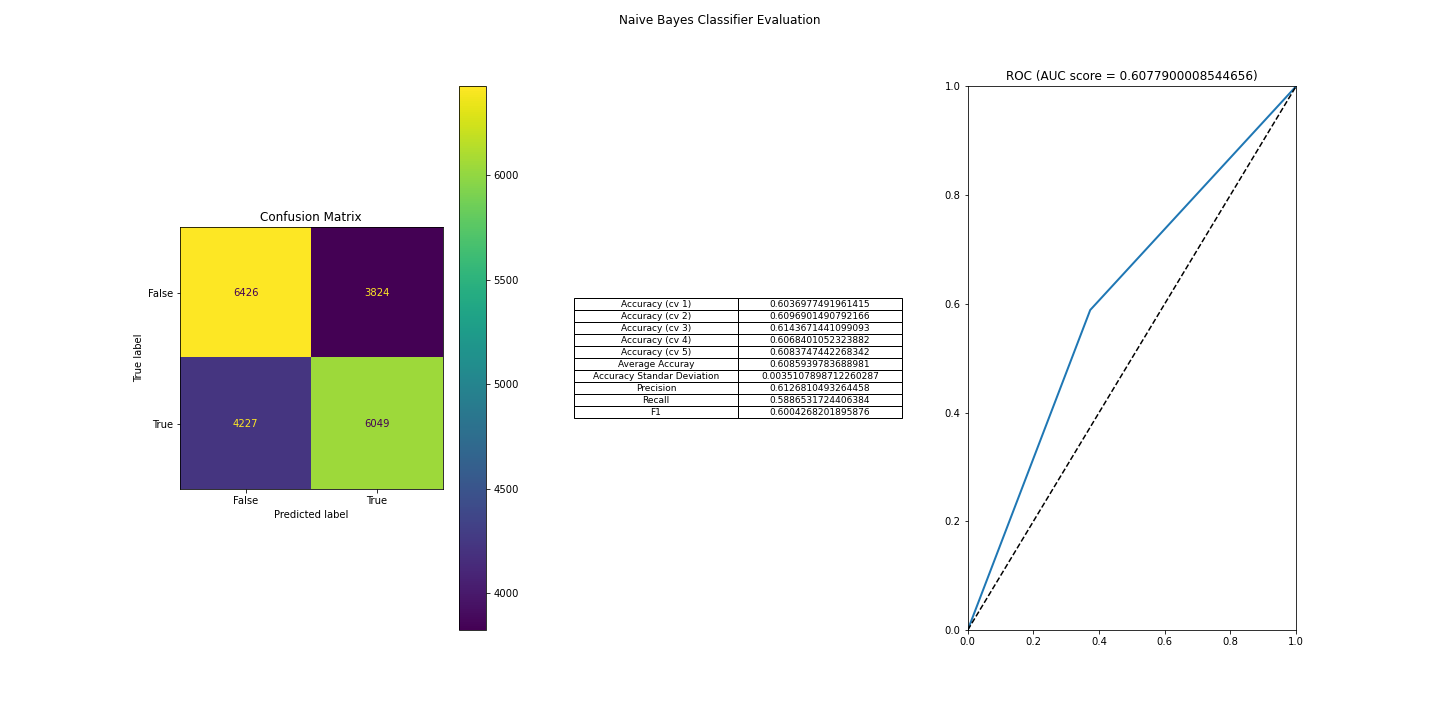
\includegraphics[scale=0.32]{img/nbc_d.png}
    \caption{Naive Bayes Classifier Evaluation}
    \label{nbc}
\end{figure}

\subsection{k-Nearest Neighbors}
The k-nearest neighbors algorithm works by classifiying an individual by
looking at its neighbors \cite{knn_wikipedia}. The classifier simply look at
the \(k\) nearest neighbors of the individual in the training population and
attributes the class that correspond the best to the neighbors (the neighbors
vote for their class, each vote is weighted either evenly accros the neighbors
or according to the distance between the individual and the voting neighbor
\cite{knn_scikit}).\\

% When trained on the balanced dataset with removed individuals, the k-Nearest
% Neighbors algorithms managed to perform worse than a random classifier (i.e.
% ROC AUC score lower than 0.5). But as soon as there are more individuals to
% learn on (with the dataset containing duplicated individuals), the algorithm
% performs very well (Figure \ref{knn}). Using cross-validation, the average
% precision is close to 0.98 and the average recall is simply 1 (with very little
% deviation in each case). This means the classifier is able to make really good
% predictions (when it finds a defective individual it is correct about 98\% of
% the times) while not missing any defective individual.\\
% The latter might be very interesting for real world application as the company
% would rather manually check a item identified as defective and find out it is
% not defective rather than missing defective ones.

According to Figure \ref{knn}, this algorithm creates a model that is close to
a random classifier. Using cross-validation, the average precision is lower
than 1\% and the average recall is lower than 2\% (with very little deviation
in each case). This means that, no matter the training set, the classifier is
no able to distinguish a defective item from a correct one.\\

\begin{figure}
    \center
    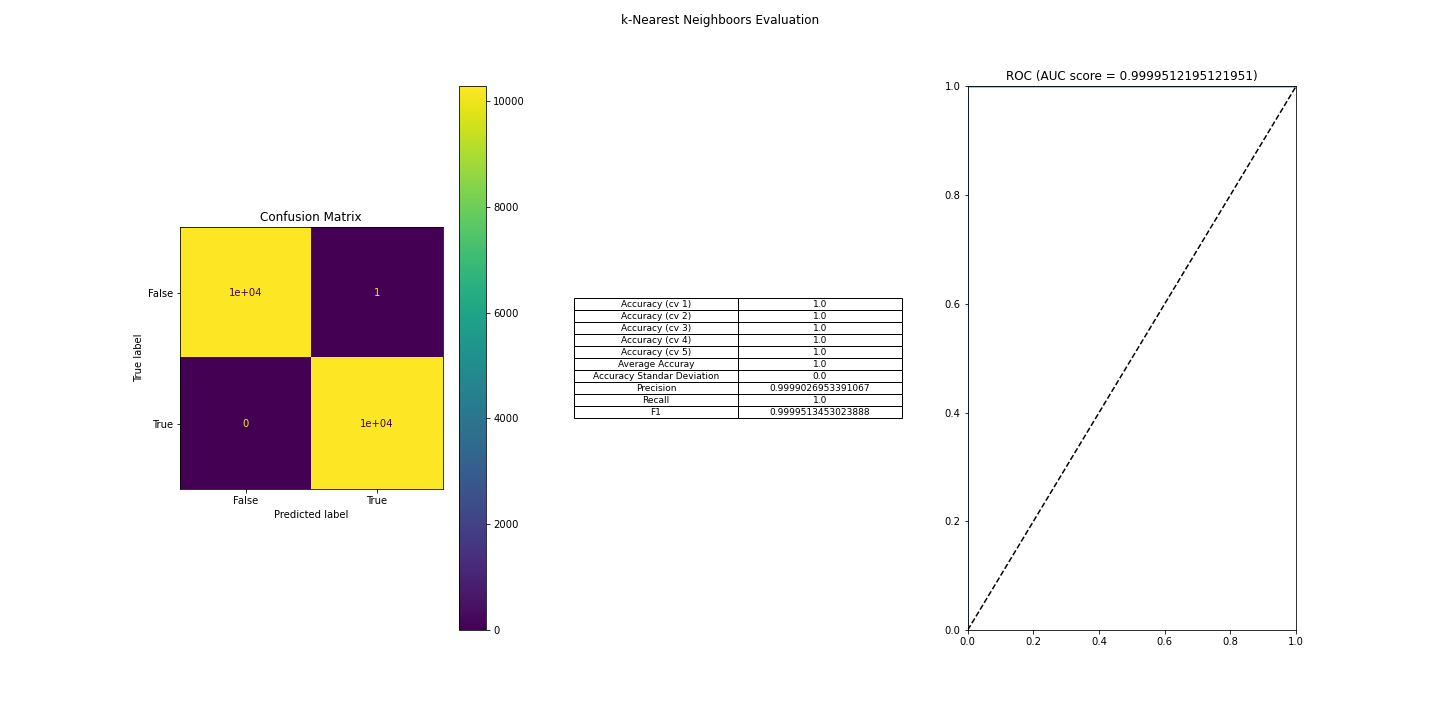
\includegraphics[scale=0.32]{img/knn_d.png}
    \caption{k-Nearest Neighbors Evaluation}
    \label{knn}
\end{figure}

\subsection{Random Forest Classifier}
Random Forest Classifier works by creating multiple Decision Trees on various
subsets of the data, the decision of the forest for classification is simply
the class that has been predicted by most of the trees \cite{rfc_wikipedia}. A
Decision Tree is built by finding the rule which devides the best the
population of each node, this can be the rule that isolate most individuals
from the same class (this method is called information gain and is based on the
concept of entropy)\cite{dtl_wikipedia}. A node cannot be devided when there
are not enough individuals (in the node or in the to-be-created child-node),
then the leaf is labeled with the class with the most representants on the
node.\\

Random Forest Classifiers have a \textit{class\_weight} attribute in
Scikit-Learn in order to address imbalance between classes\cite{rfc_scikit}.
However it seemed to perform worse than training the forest with the dataset
containing duplicates (Figure \ref{rfc_w}). The ROC AUC score on Figure \ref{rfc_d} shows
just-above-random results. But looking at the precision and recall shed the light on a useless model. Not being able to detect any defective item makes it a very bad candidate.\\

\begin{figure}
    \center
    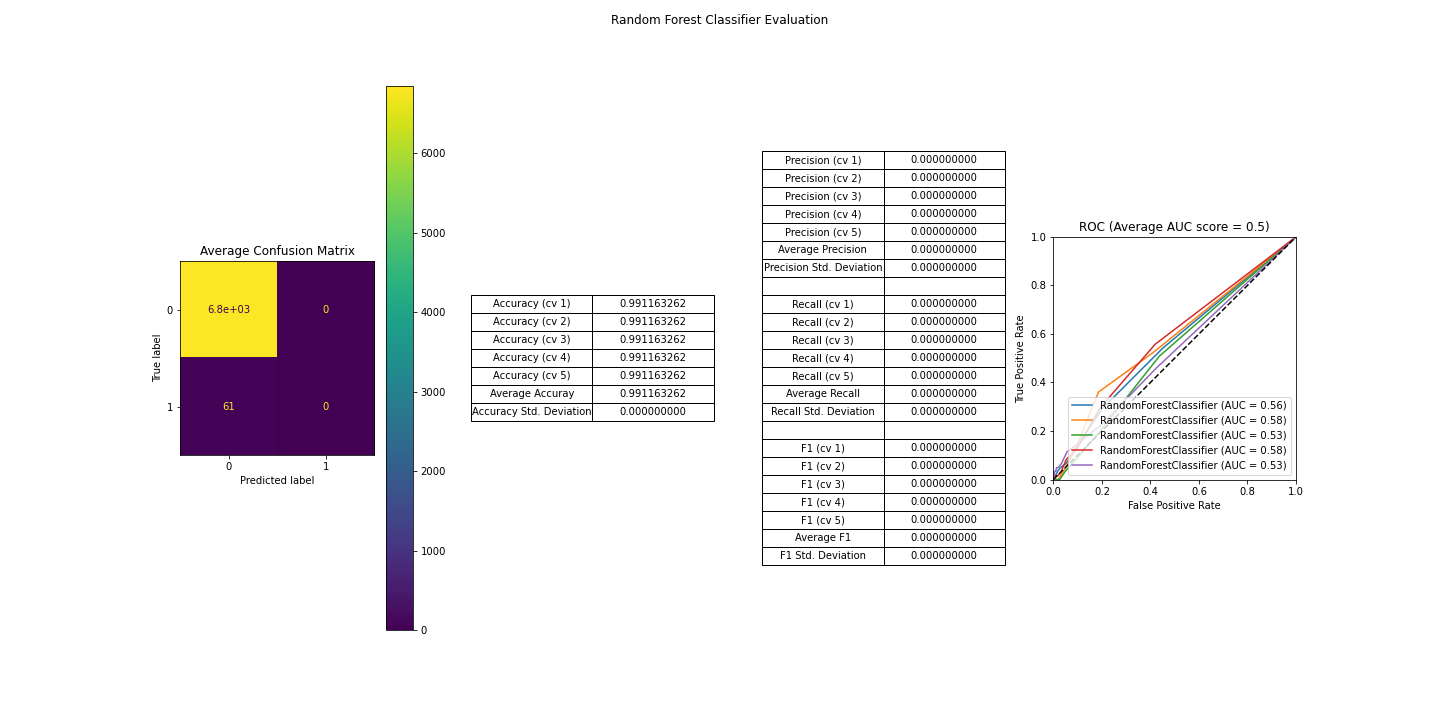
\includegraphics[scale=0.32]{img/rfc_w.png}
    \caption{Random Forest Classifier Evaluation (with \textit{class\_weight}
        set to \textit{"balanced"} )}
    \label{rfc_w}
\end{figure}

\begin{figure}
    \center
    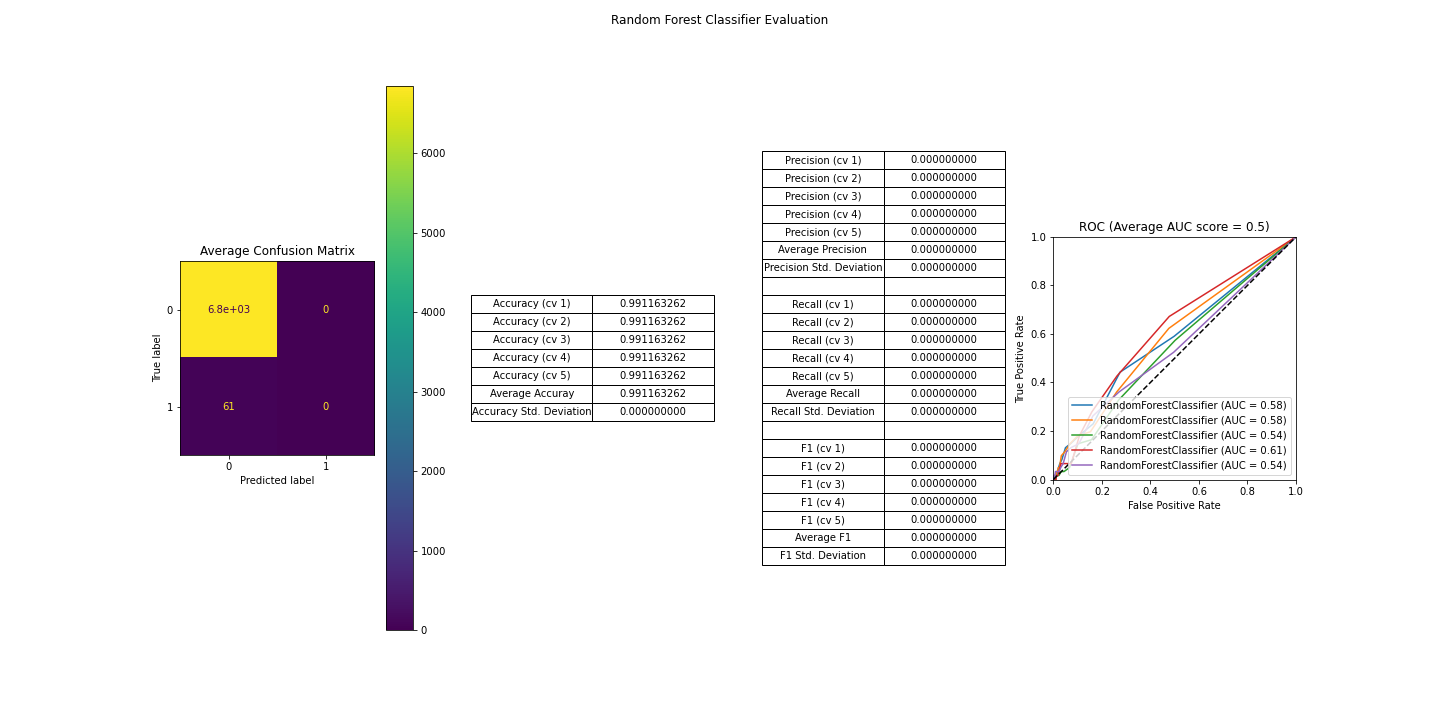
\includegraphics[scale=0.32]{img/rfc_d.png}
    \caption{Random Forest Classifier Evaluation}
    \label{rfc_d}
\end{figure}

\subsection{Multilayer Perceptron}
Multilayer Perceptron is part of the non-linear supervised learning branch.
MLPs are characterised by iterative learning on the perceptrons present in the
network layers \cite{mlp_scikit}. Several arguments can be adjusted in order to
modify the shape and parameters of the MLP:\\

\begin{itemize}
    \item hidden\_layer\_sizes : number of neurons in each hidden layer
    \item activation : activation function for the hidden layer
    \item solver : solver for weight optimization
    \item alpha : strength of the L2 regularization term
    \item batch\_size : size of minibatches for stochastic optimizers
    \item learning\_rate : learning rate schedule for weight updates
    \item max\_iter : maximum number of iterations
    \item random\_state : random number generation for weights and bias
          initialization
    \item early\_stopping : early stopping indicator (terminate training when
          validation score is not improving)
    \item n\_iter\_no\_change : maximum number of epochs to not meet tolerance
          for the optimization improvement
\end{itemize}

The MLP that gave the best results is composed of an input layer with 12
perceptrons and an output layer with one perceptron.

It is important to note that in the sklearn module, it is not possible to
modify the cost function, which by default is the LogLoss function. The Logloss
function minimizes the inverse of the log likelihood:

\[LL = -\frac{1}{n}\sum_{i=0}^{n} \left( y_{i} \log (p_{i}) + (1-y_{i}) \log
    (1-p_{i}) \right) \]

The loss is calculated for each batch, \(n\) is the value of the batch size,
\(y_i\) is the output of the neural network and \(p_i\) is the associated
probability.\\

There is no method to anticipate the most relevant hyperparameters. The only
way is to test several combinations by changing only one hyperparameter at a
time and to observe the performance of the resulting network on our data. The
best parameters obtained during testing are presented in Figure
\ref{mlp_param}.

Figure \ref{mlp_d} shows decieving results. Despite the time invested in training the network, it is not able to perform better than a random classifier on average (ROC AUC score below 0.5 on Figure \ref{mlp_d}). This is another bad candidate for the problem.\\

\begin{figure}
    \begin{center}
        \begin{tabular}{|c|c|}
            \hline
            \textbf{Hyperparameters} & \textbf{Selected value}     \\ \hline
            hidden\_layer\_sizes     & (200,150,100,50)            \\ \hline
            activation               & hyperbolic tangent          \\ \hline
            solver                   & stochastic gradient descent \\ \hline
            alpha                    & \(10^{-3}\)                 \\ \hline
            batch\_size              & 128                         \\ \hline
            learning\_rate           & adaptive                    \\ \hline
            max\_iter                & 2000                        \\ \hline
            random\_state            & 1                           \\ \hline
            early\_stopping          & True                        \\ \hline
            n\_iter\_no\_change      & 6                           \\ \hline
        \end{tabular}
    \end{center}
    \caption{Best parameters for the MLP}
    \label{mlp_param}
\end{figure}

\begin{figure}
    \centering
    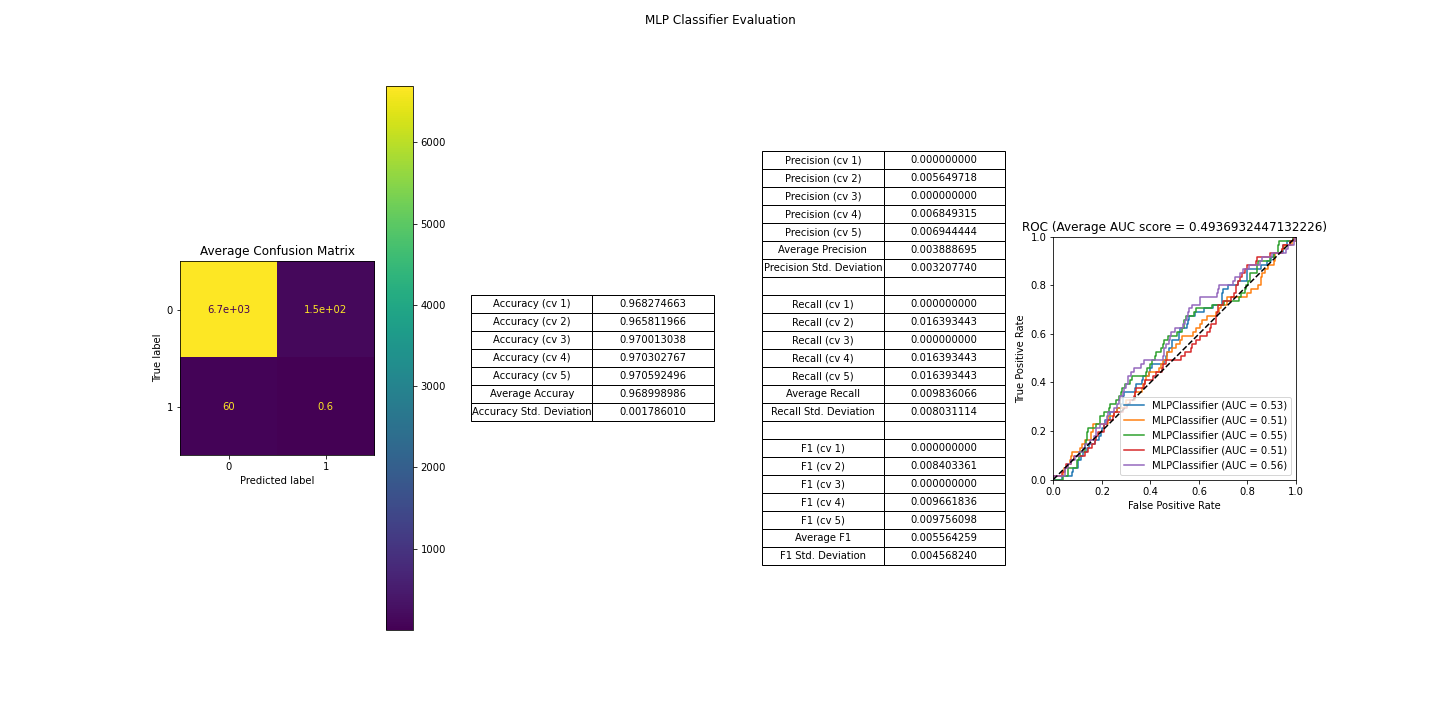
\includegraphics[scale=0.32]{img/mlp_d.png}
    \caption{MLP Classifier Evaluation}
    \label{mlp_d}
\end{figure}

\subsection{Novelty Detection}
Anomaly or Novelty detection is a subset of machine learning particularly
fitting to unbalanced class problems \cite{novel_scikit}. Knowing only the data
and the estimated proportion of defects, the model will train itself and learn
what a valid individual is supposed to look like \cite{novel_yt}. It will then
be able to classify new individuals: everything that is different than a valid
item will be classified defective. Consequently, this means that the model is
able to detect defects that are not depicted in the training datset. This
ability might be very be a advantge for this application as the model will stay
relevant even when new defects occur. For instance, the tools on the assembly
line will probably wear down leading to the apparition of new defects.\\

The model choosen for novelty detection is a One Class SVM classifier \cite{osvm_scikit} with a radial basis function kernel. This classifier did notn perform well during testing with an average precision lower than 1\% but it has an impresive average recall of 0.95 with only 2\% standard deviation during cross validation.\\

\begin{figure}
    \centering
    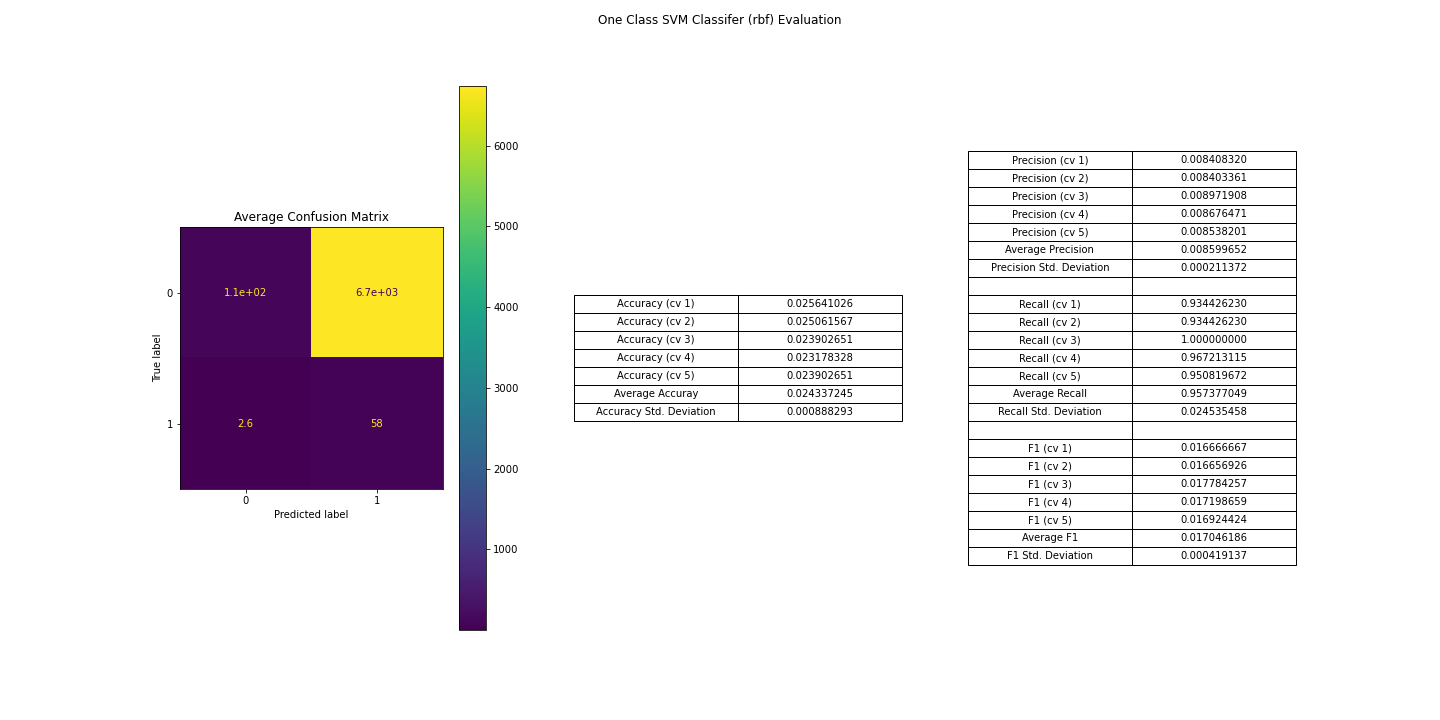
\includegraphics[scale=0.32]{img/osvm_rbf_d.png}
    \caption{One Class SVM Classifier Evaluation}
    \label{osvm_d}
\end{figure}